

%----------------------------------------------------------------------
%RESUMEN
El objetivo de este capítulo es introducir los conceptos de: 1) qué es la seguridad de la información y su importancia; 2) cómo se involucra la seguridad en la fase de diseño de un sistema; 3) qué son los patrones de seguridad y 4) los métodos de medición de seguridad que existen, haciendo énfasis los que se refieren a patrones de seguridad.

%----------------------------------------------------------------------
%SEGURIDAD DE LA INFORMACIÓN 
\section{¿Qué es seguridad de la información?}\label{sec:segInfo}

La seguridad de la información tiene el propósito de proteger la información, debido a que la información forma parte de los activos de cualquier organización \cite{peltier2016information}.  

\vspace{0.3cm}
%Federal Information Security Management Act

La Ley Federal de Seguridad de la Información (FISMA por sus siglas en inglés) define tres objetivos de seguridad, tanto para la información como para sistemas de información \cite{Sta11,StaTec0409}: 

\begin{description}
	\item [Confidencialidad]. Mantener restricciones sobre el acceso y revelación de información. Este término incluye dos conceptos:
		\begin{itemize}[noitemsep]
			\item Confidencialidad de datos: Asegurar que la información privada o confidencial no está revelada ante individuos no autorizados.
			\item Privacidad: Asegurar que la información revelada a los individuos sea relacionada con éste.
		\end{itemize} 
	
	\item [Integridad].  Prevenir de la modificación o destrucción de la información, incluyendo el no repudio de la información y autenticación. Este término incluye dos conceptos:
	\begin{itemize}[noitemsep]
			\item Integridad de datos: Asegurar que la información y los programas cambian únicamente por una solicitud autorizada o específica.
			\item Integridad del sistema: Asegurar que un sistema modifica su funcionamiento por cambios autorizados, libre de un cambio no autorizado.
		\end{itemize} 
	
	\item [Disponibilidad]. Asegurar el acceso y uso de la información siempre y cuando sea autorizado, es decir, que el sistema trabaja apropiadamente y no existe una denegación de servicio a usuarios autorizados. 
	
\end{description}

Proteger la información implica generar controles que preserven la integridad, disponibilidad y confidencialidad de los datos, éstos tres conceptos son conocidos como el triángulo CIA (\textit{Confidentiality, Integrity and Availability}). No obstante, existen otras definiciones como la presentada en ISO/IEC 13335 que abarca además del triángulo CIA los objetivos de Responsabilidad, Autenticidad y Fiabilidad \cite{Val19}.

\begin{figure}[h!]
  \centering
    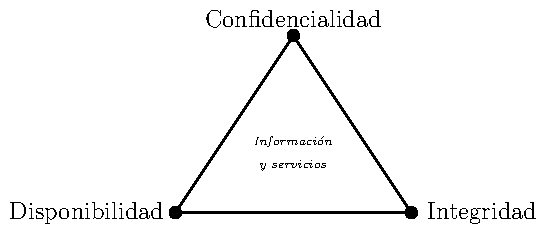
\includegraphics[scale=1]{Imagenes/ciaObj.eps}
    \caption{Triángulo de objetivos de seguridad \textit{CIA} \cite{Sta11}.}
    \label{diagrama-tr1}
\end{figure}	

\vspace{0.3cm}

En \cite{Ace1709} se definen cinco categorías en las que se extrapolan los objetivos de negocio en objetivos de seguridad, como se muestra a continuación:

\begin{itemize}[noitemsep]
	\item \textbf{Seguridad con prioridad alta}. Determina qué es lo que significa \textit{disponibilidad} para el negocio.
	\item \textbf{Seguridad persistente}. Relacionada con el término de \textit{integridad}, que incluye la retención o destrucción de la información de acuerdo con las políticas y objetivos de negocio.
	\item \textbf{Calidad de la información}. Relacionada con la \textit{integridad}, que incluye precisión, relevancia y consistencia de los repositorios. 
	\item \textbf{Control de acceso}. Se asegura que lo referente a la \textit{confidencialidad} (protección de la información) sea clara para el negocio. 
	\item \textbf{Seguridad técnica}. Cubre la parte de arquitectura de los sistemas de información y el impacto de éstos sobre el negocio. 
\end{itemize}



Proteger la información es de importancia para una organización, por ejemplo \cite{WhiMat12}: 

\begin{enumerate}[noitemsep]
	\item \textbf{Proteger la funcionalidad de la organización}. Tiene un impacto en términos de negocio y dinero, ya que podría afectar su funcionalidad.
	\item \textbf{Permitir que las aplicaciones funcionen de forma segura}. Cuando la operación de la organización depende directamente de las aplicaciones, su impacto radica en que la organización provea del servicio que ofrece de manera correcta y eficiente.
	\item \textbf{Proteger los datos que la organización recolecta y utiliza}. Si los datos no están protegidos, una organización pierde prestigio ante sus clientes, ya que no brindan garantía de que la información está siendo almacenada o manipulada de manera correcta. 
	\item \textbf{Salvaguarda los bienes tecnológicos de la organización}. Los bienes tecnológicos apoyan a que una organización crezca y consiga sus objetivos. Por esto, es de importancia que se salvaguarden. 
\end{enumerate}


Para proteger la información se requieren políticas adecuadas. Las políticas de seguridad de la información son un conjunto de criterios descritos en un documento, que sirven para proteger los sistemas y asegurar la información sensible de una organización. Los documentos sobre este tipo se dividen en políticas, estándares, procedimientos, bases y guías, las cuales se detallan a continuación \cite{peltier2016information,Lan17}: 

\begin{itemize}[noitemsep]
\item \textbf{Las políticas de seguridad de la información} son emitidas para cubrir las expectativas sobre seguridad en los sistemas y ambientes de los usuarios. Se dividen en cuatro niveles: 

\begin{enumerate}[noitemsep]
	\item Organizacional
	\item Programa de seguridad
	\item Usuarios
	\item Sistema y control
\end{enumerate}

\item \textbf{Los estándares de seguridad de la información} son requisitos más detallados que abordan la selección de metodologías, técnicas y equipos, especificando algún elemento de las políticas de seguridad. Tienen como característica ser obligatorios para todos dentro de la organización.

\item \textbf{Las guías} también son requisitos detallados, con la diferencia de que no son obligatorios para la organización, más bien son sugerencias de seguridad.

\item \textbf{Las bases o puntos de referencia} son los controles de seguridad mínimos que debe cumplir la organización. Detallan los equipos, aplicaciones, configuraciones o actividades relacionados con el control de seguridad en la organización.

\item \textbf{Los procedimientos} son instrucciones paso a paso de cómo implementar los controles de seguridad definidos en las cuatro políticas anteriores. Principalmente definen el quién y cómo de la aplicación de la seguridad. 

\end{itemize}

La seguridad de la información se divide en las siguientes áreas \cite{jacobs2015engineering}:

\begin{itemize}[noitemsep]
	\item \textbf{Evitar riesgos}. Identifica el valor y riesgo de cada componente de un sistema, incluyendo estrategias para minimizar daños.
	\item \textbf{Disuasión}. Involucra directamente al personal de una empresa, intenta persuadir a éstos antes de realizar una acción que perjudique a un sistema.  
	\item \textbf{Prevención}. Son los procedimientos que se efectúan para determinar qué necesita protección, quién debe tener accesos y quién es responsable de ciertas actividades para mantener un sistema seguro.
	\item \textbf{Detección}. Aquí se aplican medidas para detectar y reconocer actividades que estén poniendo en riesgo al sistema.
	\item \textbf{Recuperación}. Posterior a un ataque, el área de recuperación se enfoca en devolver al sistema a un estado estable. Esto se realiza mediante respaldos de información, funciones para legitimar a los usuarios que van a acceder de nuevo al sistema, etc. 
\end{itemize}

Dado que un sistema de información crea, procesa, almacena, transmite y/o destruye información, se considera que es seguro si está preparado para minimizar amenazas que comprometan la integridad, confidencialidad y acceso de este recurso. Pensar que un sistema es absolutamente seguro no es completamente correcto, ya que la existencia de amenazas no contempladas siempre está latente \cite{Nom97,RusSrLeh91}.

%----------------------------------------------------------------------
% AMENAZAS A SISTEMAS DE INFORMACIÓN 

\section{Amenazas a sistemas de información}\label{sec:amenazas}

Se denomina amenaza en los sistemas de información a cualquier acción que dañe o comprometa un recurso como hardware, software, bases de datos, datos, archivos o la red física del sistema. Para que un sistema sea propenso a amenazas, debe existir una vulnerabilidad que se interpreta como una debilidad en el diseño o en el desarrollo del sistema \cite{KimSol18}. 

\vspace{0.3cm}

Actualmente existen métodos que clasifican las amenazas bajo ciertos criterios. Las clasificaciones permiten identificar y entender las características de las amenazas con el objetivo de proteger a los recursos de una organización. Las dos principales clases en las que se dividen estos métodos son basados en técnicas de ataque y basados en el impacto de las amenazas \cite{JouRabAis14,gupta2016handbook}.

\subsection{Modelos basados en técnicas de ataque}

En esta clasificación se identifican las amenazas a través de especificaciones \cite{gupta2016handbook}. 

\begin{itemize}[noitemsep]
	\item \textbf{Análisis paso a paso}. Este modelo organiza las amenazas en: 1) amenazas de red, 2) amenazas de host y servidor y 3) amenazas de aplicación. La forma en la que se realiza la clasificación es posible cubrir todas las amenazas, aunque su debilidad es que no provee esquema de clasificación mutuamente exclusiva, por ejemplo, un ataque de DoS (\textit{Denial of Service}) afecta tanto a servidores como a la red.
	\item \textbf{Modelo híbrido}. Considera tres criterios principales: 1) frecuencia de la amenaza, 2) área donde la amenaza se focaliza y 3) origen de la amenaza. En particular, esta clasificación se considera dinámica, por ejemplo, una amenaza que tiene una frecuencia alta de aparición puede generar pocas pérdidas, o una amenaza que se origine fuera de la organización es más probable que dañe más que una interna.
	\item \textbf{Modelo piramidal}. Se basa en tres factores que identifican las amenazas de alto riesgo en los sistemas de información que son: 1) ¿cuánto sabe el atacante sobre el sistema?, 2) área crítica y 3) pérdidas. Esta clasificación permite identificar las partes vulnerables del sistema y las áreas críticas donde puede afectar una amenaza. Una desventaja es que no incluye el impacto de la amenaza. 
\end{itemize}


\subsection{Modelo basados en el impacto de las amenazas}

Los modelos basados en vulnerabilidades o impacto de las amenazas son clasificaciones que agrupan las amenazas del mismo tipo, de las que son más relevantes en impacto y más conocidas \cite{gupta2016handbook}.

\begin{itemize}[noitemsep]
	\item \textbf{STRIDE}. STRIDE son las siglas de \textit{Spoofing, Tampering, Repudiation, Information Disclosure, Denial of Service, Elevation of Privilege}. Es una clasificación que contempla tanto amenazas de red, host y aplicación. Una de las características de este modelo es que a cada amenaza le asigna una propiedad de seguridad que es violada y donde impacta.
	\item \textbf{Modelo ISO}. El ISO 7498-2 hace una clasificación en cinco grupos: 1) destrucción de información y/o recursos, 2) modificación de la información, 3) pérdida de información y/o recursos, 4) exposición de información y 5) interrupción de servicios. Este modelo presenta una clasificación mutuamente exclusiva, aunque no cubre las consecuencias de todos los ataques. 
	\item \textbf{Misuse activities}. Es un modelo para identificar amenazas en el sistema. Utilizan diagramas de actividades diseñados en UML, sobre los que se plasman las actividades desde el punto de vista de un actor hostil.
\end{itemize}

La gran ventaja de estos modelos de clasificación es que desde la fase de diseño se consigue saber cuáles amenazas afectarían al sistema que se va a desarrollar. 

\subsubsection*{Descripción del modelo \textit{Misuse activities}}

En el artículo ``\textit{Eliciting security requirements through misuse activities}'' \cite{BraFerVan08} se propone la obtención de un modelo de amenazas utilizando \textit{misuse activities}. Una de las características de este modelo es que se enfoca en las amenazas relacionadas directamente con las actividades del sistema desde la fase de diseño. A continuación, se describe cómo obtener el modelo de amenazas en un sistema. Este modelo parte de diagramas de caso de uso\footnote{Los diagramas de secuencia complementan la descripción textual de los diagramas de caso de uso, por lo tanto no son indispensables para el modelado.} en UML, de los cuales se obtiene el diagrama o los diagramas de actividades del sistema que se está diseñando. Sobre el diagrama de actividades se realiza un análisis para descubrir las amenazas relacionadas con las actividades que ejecuta el sistema (este proceso se hace con cada caso de uso del sistema). En este análisis hay tres aspectos que se consideran:

\begin{enumerate}[noitemsep]
	\item \textbf{Escenarios del sistema}. Se deben encontrar todos los posibles escenarios del sistema de los casos de uso, inclusive se debe contemplar el análisis de secuencias de casos de uso. El análisis de los diagramas de actividades permite identificar las amenazas en el flujo del negocio.
	\item \textbf{Atributos de seguridad}. Cada actividad del diagrama de actividades es analizada con respecto a los objetivos de seguridad.
	\item \textbf{Origen de la amenaza}. Para cada actividad se analiza de donde proviene el ataque:
	\begin{itemize}[noitemsep]
		\item Atacante interno autorizado: Persona que tiene acceso al sistema y tiene los permisos para realizar la actividad analizada.
		\item Atacante interno no autorizado: Persona que pertenece a la empresa, pero no tiene permiso para realizar la actividad analizada.
		\item Atacante externo: Persona ajena a la empresa y no tiene permiso de realizar la actividad analizada.
	\end{itemize}
\end{enumerate} 

Para analizar cada actividad se debe pensar en \textit{``qué mal uso se puede realizar en <actividad> por <origen de amenaza> que compromete el <objetivo de seguridad> del <dato a proteger>''}. Cada posible amenaza se plasma en una plantilla (definida en el artículo) que proporciona un panorama de las amenazas a las que está expuesto el sistema. 

%----------------------------------------------------------------------
% SEGURIDAD EN LA FASE DE DISEÑO DE UN SISTEMA 
\section{Seguridad en la etapa de diseño de un sistema}\label{sec:segDiseño}

En la etapa de diseño se define la arquitectura de software o hardware, componentes, módulos, interfaces y datos de un sistema que en conjunto satisfacen requerimientos específicos \cite{Weik2001}. %verificar si son "datos"

\vspace{0.3cm}

Al realizar un nuevo sistema (o una mejora a uno existente), se espera provea un beneficio. La mayoría de los sistemas contienen procesos confidenciales o información sensible de la empresa. Por lo tanto, para mantener una postura de seguridad se deben tomar en cuenta las técnicas de seguridad preventivas que eliminen las incertidumbres del comportamiento del sistema en fases posteriores \cite{BazLim07}. Un sistema al cual no se le haga una revisión de seguridad desde la etapa de diseño podría presentar los siguientes problemas \cite{BazLim07}:

\begin{itemize}[noitemsep]
	\item Exposición de la información o exhibir la postura de seguridad de la empresa.
	\item En una auditoria, la falta de controles de seguridad en un sistema se convertiría en una evaluación negativa. 
	\item Tomar una medida correctiva ante un problema de seguridad en un sistema ya desarrollado se torna perjudicial para la empresa, principalmente por el costo que conlleva la reparación del problema (en términos de recursos y tiempo) y la dificultad de implementarla (una ingeniería inversa de seguridad se extrapola a un sistema inseguro). 
\end{itemize}

Existen guías que incluyen seguridad en el diseño de un sistema. Éstas se expresan en forma de buenas prácticas, principios, políticas, reglas, regulaciones y estándares. El objetivo de las guías es saber qué tan seguro es el diseño de un sistema. Las dos principales se describen a continuación \cite{Mjo12}:
\begin{itemize}[noitemsep]
	\item \textbf{Principios de diseño de seguridad}. Los principios de diseño de seguridad son reglas probadas para incrementar la seguridad de un sistema, las cuales son aplicadas a problemas específicos. Son identificados durante la etapa de análisis mediante modelado de amenazas. Utilizar estos principios proporciona la ventaja que al identificar una debilidad en el diseño del sistema, se pueden tomar decisiones con respecto a la arquitectura e implementación. 
	
	\item \textbf{Patrones de seguridad}. Los patrones de seguridad son una solución a un problema de seguridad recurrente, que alienta al rehuso efectivo para construcción de sistemas más robustos. Estos ayudan a manejar un solo requerimiento que es la seguridad de un sistema. 
\end{itemize}

Para incluir la seguridad en el diseño deben existir requisitos de seguridad. El NIST (\textit{National Institute of Standards and Technology} por sus siglas en inglés) en el FIPS 200 muestra un listado de los requisitos de seguridad mínimos que se deben considerar para cualquier sistema de información al que se le quiera incluir seguridad. Al igual que en el FIPS 200, Eduardo B. Fernández ha realizado un listado típico de requisitos de seguridad, los cuales se muestran en la Tabla \ref{poliSeg}

\vspace{0.3cm}

Las políticas de seguridad de una empresa también son considerados como requisitos de seguridad de un sistema o pueden agregarse dichas políticas a un listado ya existente. Eso depende del diseño del sistema. 

\begin{table}[!ht]
\caption{Listado de políticas de seguridad típicas \cite{Fer1908}}
\begin{center}
\scriptsize
\begin{tabular}{|m{0.5cm} |m{3.5cm}|m{10cm}|}
	\hline
	\cellcolor{lightgray}\textbf{\#}&\cellcolor{lightgray}\textbf{Política} & \cellcolor{lightgray}\textbf{Descripción}\\ \hline
	P1 & Sistemas abiertos/cerrados & En los sistemas cerrados nadie puede acceder a los recursos a menos que tenga acceso explícito; en los sistemas abiertos todos tienen acceso a menos que exista negación explícita.\\ \hline
	P2 & Privilegios mínimos & Personas o entidades son autorizadas a acceder a los recursos para realizar solo sus funciones. \\ \hline
	P3 & Autorización & Reglas explícitas deben usarse para quién puede usar qué recursos y cómo. \\ \hline
	P4 & Obligación & El acceso a los recursos se da únicamente si se ejecutan acciones antes o después de otorgar el acceso.\\ \hline
	P5 & Separación de responsabilidades & Funciones críticas deben asignarse a más de una persona o sistema. \\ \hline
	P6 & Auditoria e Inicio de sesión & Define como examinar y auditar los logs de acceso al sistema. Incluye cuánto tiempo deben almacenarse los logs y cada cuánto se deber examinar.\\ \hline
	P7 & Autenticación de transacciones & Cualquier intercambio de información debe ser autenticada por ambos lados. \\ \hline
	P8 & Control centralizado / descentralizado & En sistemas descentralizados cada unidad o división tienen sus propios administradores y autoridades para definir políticas internas que no violen las políticas globales de la empresa.\\ \hline
	P9 & Propiedad y administración & Separar la administración de los datos con el uso de éstos. \\ \hline
	P10 & Responsabilidad individual & Personas o procesos deben ser identificados de manera única y sus acciones deben ser registradas y revisadas. \\ \hline
	P11 & Roles & Cada rol tiene diferentes privilegios sobre los datos que correspondan con las actividades que realizan. \\ \hline
	P12 & Control de acceso dependiente de los datos & Controlar el acceso a datos nombrados y a clases nombradas incluyendo sus instancias. \\ \hline
	P13 & Control de acceso dependiente del contenido & El acceso a los datos depende del registro solicitado.\\ \hline
	P14 & Control de acceso dependiente del contexto & El acceso a los datos depende en qué otra información se está solicitando. \\ \hline
	P15 & Control de acceso dependiente de la historia & Se debe considerar todas o un conjunto de las solicitudes anteriores para otorgar el acceso.  \\ \hline
	P16 & Otorgar o denegar privilegios & Un usuario que tenga los derechos puede otorgar o quitar derechos a su discreción. \\ \hline
	P17 & Obligaciones& Un usuario obtiene privilegios sobre el sistema pero no puede otorgarlos a otros. \\ \hline
	P18 & Privilegios multinivel & Los usuarios son clasificados en niveles y sus privilegios dependen del nivel.  \\ \hline
	P19 & Verificación del origen de la información & Verificar de dónde procede la información\\ \hline
\end{tabular}
\label{poliSeg}
\end{center}
\end{table}

\normalsize


%En la lista siguiente se muestran algunos de los requisitos de seguridad que describe el FIPS 200 \cite{StaTec0609}:
%
%\begin{itemize}
%	\item Control de Acceso
%%	\item Conocimiento y Entrenamiento
%	\item Auditoria y Gestión de roles
%	\item Certificación, Acreditación y Evaluaciones de seguridad
%	\item Administración de configuraciones 
%%	\item Planeación ante contingencias
%	\item Identificación y Autenticación
%	\item Responsable ante incidentes
%%	\item Mantenimiento
%%	\item Protección de medios de comunicación
%%	\item Protección de elementos físicos y entorno de trabajo
%%	\item Personal de seguridad
%	\item Evaluaciones de riesgo
%	\item Adquisición de sistemas y servicios
%	\item Protección de sistemas y comunicaciones
%	\item Sistemas e Integridad de la información
%\end{itemize}





%----------------------------------------------------------------------
%PATRONES DE SEGURIDAD
\section{Patrones de seguridad}\label{sec:patSeg}

La definición que Fernández da sobre los patrones de seguridad es \cite{SchFerHyb06}:

\begin{quote}
\textit{``Un Patrón de Seguridad describe la solución a un problema de seguridad recurrente que se genere dentro de un contexto específico y provee un esquema de solución genérico.''}
\end{quote}

Una de las razones por las cuales los patrones de seguridad son exitosos es que dan una solución que puede ser usada en diferentes situaciones y adaptada para resolver un problema nuevo dentro del mismo contexto. Capturan la solución y su relación con el problema planteado de manera rápida y accesible. Cabe resaltar que un Patrón de Seguridad se encuentra directamente relacionado con la amenaza y no con la vulnerabilidad \cite{SchFerHyb06}. 

\vspace{0.3cm}

Lo que diferencia a los patrones de seguridad de los patrones tradicionales es el contexto en que se desenvuelven. Los patrones de seguridad tienen una estructura que se compone de los siguientes elementos esenciales: 1) Nombre, 2) Contexto, 3) Problema y 4) Solución.  Las características de estos elementos se describen a continuación \cite{SchFerHyb06}:

\begin{enumerate}[noitemsep]
	\item \textbf{Nombre}. Es el nombre descriptivo del patrón de seguridad.
	\item \textbf{Contexto}. Describe el ambiente y las condiciones en las que el problema de seguridad está ocurriendo.
	\item \textbf{Problema}. Éste se presenta cuando el sistema de software se encuentra en una situación de vulnerabilidad, siendo esta vulnerabilidad una puerta que de motivo a ataques. El problema abarca todos los niveles en la arquitectura del sistema de software. 
	\item \textbf{Solución}. Está fuertemente ligada con el contexto. Se diseña para uno o más niveles de la arquitectura del sistema de software y también puede abarcar procesos. La solución estará enfocada según el contexto a la prevención, detección o reacción a un ataque o posible vulnerabilidad.
\end{enumerate}

Algunas de las ventajas del uso de patrones de seguridad en el desarrollo de sistemas son \cite{SchFerHyb06}:

\begin{itemize}[noitemsep]
	\item Encapsulan el conocimiento básico de seguridad de una forma estructurada y entendible. 
	\item Ayudan a mejorar la integración de la seguridad en los sistemas y empresas.
	\item Con su uso se extiende la seguridad a todos los niveles de la arquitectura de un sistema.
\end{itemize}

Clasificar los patrones de seguridad sirve para una selección e identificación más adecuada y precisa. Actualmente se han identificado varias clasificaciones con base en criterios o atributos de los patrones. La Tabla \ref{clasiPatrones} se muestra una recopilación de las clasificaciones más utilizadas por los investigadores \cite{PonShiKre16}.
\begin{table}[!tb]
\scriptsize
\begin{center}
\begin{tabular}{ |m{3.5cm}|m{4cm}|}
\hline
\cellcolor{lightgray}\textbf{Clasificación} &\cellcolor{lightgray} \textbf{Atributos} \\
\hline
 
 \multirow{5}{*}{Propósito} &  Estructural \\ \cline{2-2}
 &  De procedimiento \\ \cline{2-2}
 & Ambiente \\ \cline{2-2}
 & Para creación\\ \cline{2-2}
 & Genéricos \\ \hline

 
 \multirow{5}{*}{Ciclo de vida del sistema} &  Arquitectónico \\ \cline{2-2}
 &  Requisitos \\ \cline{2-2}
 & Diseño \\ \cline{2-2}
 & Análisis \\ \cline{2-2}
 & Implementación \\ \hline

\multirow{9}{*}{Objetivos de seguridad} &  Confidencialidad \\ \cline{2-2}
 &  Integridad \\ \cline{2-2}
 & Responsabilidad \\ \cline{2-2}
 & Autenticación \\ \cline{2-2}
 & Disponibilidad \\ \cline{2-2}
 & Control de acceso \\ \cline{2-2}
 & Identificación \\ \cline{2-2}
 & No repudio \\ \cline{2-2}
 & Transmisión de datos segura\\ \hline
\end{tabular}
\caption{Clasificación de patrones de seguridad obtenida de \cite{PonShiKre16}}
\label{clasiPatrones}
\end{center}
\end{table}

\normalsize

\vspace{0.3cm}

Un listado con algunos patrones de seguridad incluidos en las clasificaciones mostradas
La lista a continuación muestra algunos patrones de seguridad incluidos en la clasificación anterior.

\vspace{0.3cm}

\textbf{Propósito} \cite{KonCamWas03,KieEldTyr06}

\begin{itemize}[noitemsep]
	\item \textbf{Estructural}. \textit{Account Lockout, Authenticated Session, Client Data Storage, Client Input Filters, Encrypted Storage, Minefield, Network Address Blacklist, Partitioned Application, Password Authentication, Password Propagation, Secure Assertion, Server Sandbox y Trusted Proxy}.
	\item \textbf{De procedimiento}. \textit{Build the Server from the Ground Up, Choose the Right Stuff, Document the Security Goals, Document the Server Configuration, Enroll by Validating Out of Brand, Enroll using Third-party Validation, Enroll with a Pre-Existing Shared Secret, Enroll without Validation, Log for Audit, Patch Proactively, Red Team the Design, Share Responsibility for Security y Test on Staging Server}.
	\item \textbf{Ambiente}. \textit{Limited View y Full View with Errors}	
	\item \textbf{De creación}. \textit{Session}
\end{itemize}

\vspace{0.3cm}

\textbf{Ciclo de vida del sistema} \cite{MelJen08}.

\begin{itemize}[noitemsep]
	\item \textbf{Arquitectónico}. \textit{Distrustful Decomposition, PrivSep (Privilege separation) y Defer to Kernel}
	\item \textbf{Diseño}. \textit{Secure Factory, Secure Strategy Factory, Secure Builder Factory, Secure Chain of Responsibility, Secure State Machine y Secure Visitor}
	\item \textbf{Implementación}. \textit{Secure Logger, Clear Sensitive Information, Secure Directory, Pathname Canonicalization, Input Validation y RAII (Resource Acquisition Is Initialization)}
\end{itemize}

\vspace{0.3cm}

\textbf{Objetivos de seguridad} \cite{ScaJooYsk06}.

\begin{itemize}[noitemsep]
	\item \textbf{Confidencialidad}. \textit{Controlled Access y Secure Data Transmission }
	\item \textbf{Integridad}. \textit{Checkpointed System, Comparator-Checked Fault-tolerant System, Input Guard, Output Guard, Secure Access Layer, Controlled Object Factory, Controlled Process Creator, Server Sandbox}
	\item \textbf{Responsabilidad}. \textit{Replicated System, Session Failover, Session Timeout, Load Balancer, Reverse Proxy}
	\item \textbf{Autenticación y No repudio}. \textit{SAP (Single Access Point) y Check Point}
	\item \textbf{Disponibilidad}. \textit{Secure Logger y Audit Interceptor}
	\item \textbf{Control de acceso}. \textit{Authentication enforcer, Authorization Enforcer, Container-Managed Security, Secure Service Facade, Application Firewall, Demilitarized Zone, Firewall y Single Access Point}
	\item \textbf{Identificación}. \textit{Credential tokenizer, Security Context, Session y Subject Descriptor}
	\item \textbf{Transmisión de datos}. \textit{Obfuscated Transfer Object, Security Association, Secure Message Router y Secure pipe}

\end{itemize}


Independientemente de la clasificación a la que pertenezcan, los patrones de seguridad entran en alguna de las cinco relaciones inter-patrones: \textit{dependencia, beneficios, alternativa, perjudiciales y en conflicto}, que muestran el impacto que tiene aplicar un patrón A junto con un patrón B \cite{ScaJooYsk06}. 

\begin{itemize}[noitemsep]
  \item[] \textbf{Dependencia}. Si el patrón A depende del patrón B, entonces es necesario el patrón B para la correcta funcionalidad de A.
  \item[] \textbf{Beneficios}. Si el patrón A se beneficia del patrón B, entonces, implementar el patrón B incrementa el valor del patrón A.
  \item[] \textbf{Alternativa}. Los patrones A y B tienen funcionalidad similar, aunque no son identicos.
  \item[] \textbf{Perjudiciales}. El patrón A se ve perjudicado al implementar el patrón B. Al ser implementados estos patrones se debe verificar que no existan dichos errores en el desarrollo.
  \item[] \textbf{En conflicto}. El patrón A entra en conflicto con el patrón B, generando inconsistencias. Este caso se da cuando se implementan dos patrones para resolver el mismo problema.
\end{itemize}

\subsection*{Ejemplo}

Un resumen del  Patrón de Seguridad \textbf{Autenticador (\textit{Authenticator})} se muestra en la Tabla \ref{resuPat}:

\begin{table}[!ht]
\caption{Resumen del patrón de seguridad \textbf{Autenticador} \cite{Fer13}}
\begin{center}
\scriptsize
\begin{tabular}{|m{3.5cm}|m{10cm}|}
	\hline
	\cellcolor{lightgray}\textbf{Característica} & \cellcolor{lightgray}\textbf{Descripción}\\ \hline
 	Descripción &   El patrón \textbf{Autenticador} permite verificar que el sujeto que intenta acceder al sistema es quien dice ser. \\ \hline

	Contexto &  Sistemas computacionales que contienen recursos que se vuelven valiosos ya que incluyen información sobre planes sobre el negocio, reportes médicos, etc. Solo se requiere que sujetos autorizados para entrar al sistema lo hagan. \\ \hline

	Problema &  ¿Cómo podemos prevenir que impostores entren a nuestro sistema? Un atacante puede intentar suplantar la identidad de un usuario legítimo para tener acceso a sus recursos. Esto es riesgoso si el usuario suplantado tiene un nivel alto de privilegios al sistema. ¿Cómo verificar que un usuario intentado acceder al sistema es legítimo? \newline
La solución a este problema debe contemplar también:\newline
\textbf{Flexibilidad}: Muchos usuarios requieren acceso al sistema y en varias unidades del sistema existen diferentes datos importantes.\newline 
\textbf{Confiabilidad}: Necesitamos autenticar usuarios de manera confiable y segura, es decir, utilizar un protocolo robusto y una manera de proteger los resultados de la autenticación.\newline
\textbf{Modificación}: Si la autenticación necesita ser modificada frecuentemente, esta se convierte en un problema. \newline
\textbf{Frecuencia}: Se debe evitar que los sujetos se autentiquen con frecuencia. 
\\ \hline

	Solución &  Utilizar un punto de acceso para recibir todas las interacciones entre sujetos y el sistema, aplicar el protocolo para  verificar la identidad del sujeto. El protocolo será simple o complejo dependiendo de las necesidades de la aplicación.\\ \hline
\end{tabular}
\label{resuPat}
\end{center}
\end{table}

\normalsize

En la Figura \ref{diag_Auth} se muestran los diagramas correspondientes al patrón anterior. La implementación del patrón contempla que existe un sistema centralizado, donde el sistema operativo controla la creación de sesiones en respuesta a una petición del sujeto (usuario). El usuario autenticado tiene permitido el acceso a los recursos de acuerdo a los derechos que tenga sobre estos.

\begin{figure}[h!]
\begin{center}
   \subfloat[Diagrama de clase]{
   \label{useCase_check}
    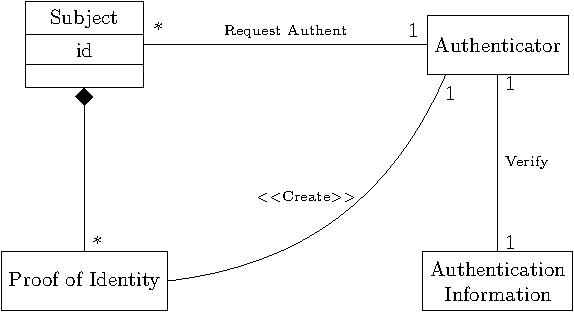
\includegraphics[width=0.4\textwidth]{Imagenes/diag_class_Authenticator_pt.eps}}
    \hspace{1cm}
  \subfloat[Diagrama de secuencia]{
   \label{actDiag_check}
    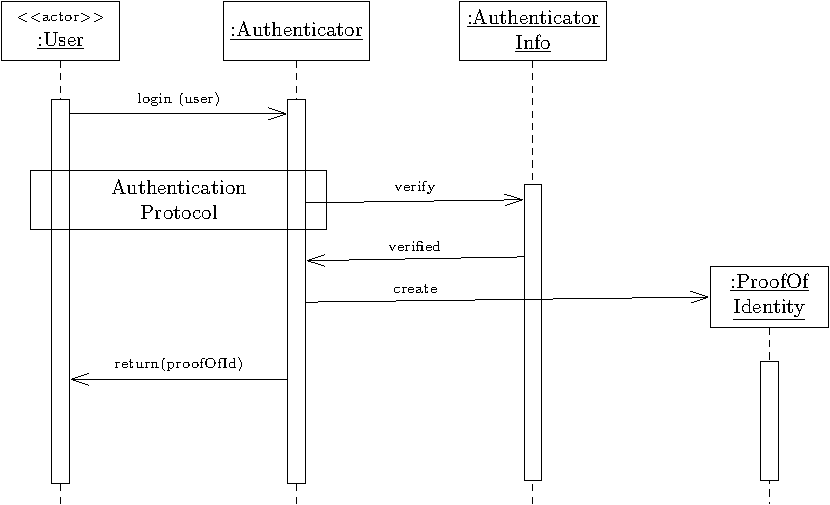
\includegraphics[width=0.5\textwidth]{Imagenes/diag_seq_Authenticator_pt.eps}}
 \caption{Diagramas sobre el patrón \textbf{Autenticador} \cite{Fer13}}
 \label{diag_Auth}
 \end{center}
\end{figure}

%MEDICION DE LA SEGURIDAD COMO PROPIEDAD DE UN SISTEMA
\section{Medición de la seguridad como propiedad de un sistema}\label{sec:medicion}

Una de las definiciones más utilizadas para medición es la propuesta por Hermann von Helmholtz en su trabajo denominado \textit{Zählen und Messen}, la cual dice \cite{Hel87}:
\begin{quote}
	\textit{Es la relación especial que puede existir entre los atributos de dos objetos y la cual designaremos con el nombre de igualdad [...]\\
	 Axioma I: Si dos magnitudes son iguales con una tercera, entonces todas ellas son iguales}
\end{quote}

Una medición determina \cite{ZalDraMcK14}:

\begin{itemize}[noitemsep]
	\item Una propiedad o atributo que representa al objeto a ser medido.
	\item Un estándar que involucra comparar dos objetos entre sí y su relación entre estos basándose en la propiedad.
	\item Un procedimiento, por el cual se colocan dos objetos bajo las mismas condiciones con el objetivo de observar el resultado y ser capaz de establecer si existe o no una ocurrencia de la relación. %Al cual se le denomina método de comparación.
\end{itemize}

Dado que la definición anterior se enfoca a medir propiedades físicas de los objetos, se requiere una adaptación de esta a la medición del software y aún más a la seguridad sobre este, ya que la seguridad no es una propiedad física, la única forma de medirla es de manera indirecta a través de sus componentes inherentes \cite{ZalDraMcK14}.

%Las mediciones de seguridad son necesarias para mejorar la toma de decisiones en el desarrollo de un sistema. Es importante medir la seguridad para predecir el comportamiento de un sistema ante amenazas.  

\vspace{0.3cm}

Una métrica tiene como objetivo proporcionar un valor escalar que describe una propiedad del sistema, en este caso particular, la propiedad analizada es la seguridad de un sistema. Las métricas de seguridad definidas y usadas en la práctica son relativas debido a que la seguridad es una propiedad que depende de percepciones.  Los resultados obtenidos de utilizar una métrica de seguridad, ayudan a la toma de decisiones en varios aspectos de seguridad, que van desde el diseño de una arquitectura, hasta la valoración de la eficiencia y eficacia de las operaciones de seguridad que está ejecutando el sistema \cite{Var1103,Jan0904}. 

\vspace{0.3cm}

Los principales usos de las métricas de seguridad se pueden incluir en las siguientes categorías:

\begin{itemize}[noitemsep]
	\item \textbf{Soporte estratégico}. Brindar garantía de seguridad en un sistema, apoya en la toma de decisiones tales como asignación de recursos, planeación y selección de productos y servicios. 
	\item \textbf{Garantía de calidad}. Para minimizar vulnerabilidades en el sistema.
	\item \textbf{Supervisión táctica}. Conocer el estado de un sistema con respecto a la seguridad apoyándose en el control y manejo de riesgos. 
\end{itemize}

Las métricas en seguridad de software se dividen en cuatro categorías \cite{Saa1603}:

\begin{enumerate}[noitemsep]
	\item Seguridad desde la perspectiva de ingeniería. Esta categoría se enfoca en verificar procesos.
	\item Seguridad desde la perspectiva de negocio. Esta categoría a su vez se divide en nivel organizacional y nivel técnico, el primero se enfoca en los riesgos económicos de mantenimiento y/o procesos y el segundo se enfoca en asegurar al sistema. 
	\item Seguridad desde la perspectiva de las características. En esta categoría se basan las métricas según la característica de seguridad a analizar. 
	\item Seguridad desde la perspectiva del sistema. Se enfoca en la parte técnica del sistema, dividiéndose en tres niveles, 1) Métricas a nivel sistema, 2) Métricas a nivel diseño y 3) Métricas a nivel código.
\end{enumerate}

%En el design level metrics se encuentran las métricas para patrones de seguridad.

\subsection{Medición de la seguridad al implementar patrones de seguridad}

Las investigaciones sobre medición del nivel de seguridad que proporcionan los patrones de seguridad se dividen en evaluaciones cuantitativas y cualitativas. Hay evaluaciones que toman de base cómo los patrones de seguridad atienden los objetivos de la seguridad de la información (Confidencialidad, Integridad y Disponibilidad), otras que se enfocan en identificar las amenazas que los patrones de seguridad resuelven.

\vspace{0.3cm}

A continuación se muestran dos metodologías que ejemplifican ambos tipos de evaluaciones a los patrones de seguridad:

\begin{enumerate}[noitemsep]
	\item En \cite{YauScaHey} se muestra una metodología que evalúa el nivel de seguridad que proporcionan los patrones de seguridad a la arquitectura de un sistema. Esta metodología selecciona un conjunto de patrones que cumplan cierto objetivo de seguridad de la arquitectura, posterior a eso, se les da un peso de acuerdo a la amenaza que mitigan y con eso obtener un valor que indique sobre las amenazas cuán segura es la arquitectura.
	\item En \cite{HalChaSte06} se muestra una metodología para evaluar las características de los patrones de seguridad para verificar el nivel de seguridad que otorgan. La selección de los patrones que analiza se basan en  tres criterios: 1) Si es una guía para construir software seguro, 2) Si contemplan hoyos de seguridad de software y 3) Los ataques que mitigan. Esta metodología contribuye a la selección del conjunto de patrones que mejor otorguen seguridad a un sistema determinado de manera cualitativa. 
\end{enumerate}

\section{Resumen}

En este capítulo se presenta una breve introducción a la seguridad de la información, la importancia de incluirla en los sistemas de software y las amenazas a las que están expuestos los sistemas. Se hace un énfasis en la inclusión de la seguridad en la etapa de diseño de un sistema, donde se explica que utilizar guías para proporcionar un nivel de seguridad a un sistema en diseño disminuye las posibilidades de una amenaza al sistema ya implementado. 

\vspace{0.3cm}

Se menciona que, los patrones de seguridad al ser parte de las guías para incluir seguridad en el diseño de un sistema, realmente otorgan un nivel de seguridad debido a la experiencia que involucra la solución propuesta ante ciertas amenazas. También, se aborda la clasificación de los patrones y las actuales definiciones de medición de la seguridad como un atributo y la importancia para mejorar la seguridad en los sistemas. 

